\documentclass{article}
\usepackage[margin=1in]{geometry} 
\usepackage{amsmath}
\usepackage[T1]{fontenc}          % change font encoding to T1
\usepackage{lmodern}  %better for visual on screen
\usepackage{graphicx}
\usepackage{float}
\usepackage{enumitem}
\usepackage{mathtools}
\usepackage{booktabs}
\usepackage{dirtree}

\makeatletter
\renewcommand*\env@matrix[1][\arraystretch]{%
	\edef\arraystretch{#1}%
	\hskip -\arraycolsep
	\let\@ifnextchar\new@ifnextchar
	\array{*\c@MaxMatrixCols c}}
\makeatother

% Used for adding Matlab Algorithms
\RequirePackage{listings}
\RequirePackage[framed,numbered]{matlab-prettifier}

\DeclarePairedDelimiter\abs{\lvert}{\rvert}%

\begin{document}
	\section{axgrid.m}
	\lstinputlisting[
	label      = {alg:lsr},
	style      = Matlab-editor,
	basicstyle = \mlttfamily,
	firstline  = 1,
	lastline   = 25,
	firstnumber= 1
	]{../axgrid.m}
	\subsection{Motivation/Concept}
	This function is used for more control on the spacing of subplots.  
	\clearpage
	\subsection{Math}
	The input parameters determine the number and spacing of the subplots, as shown below:
	\begin{figure}[H]
		\centering
		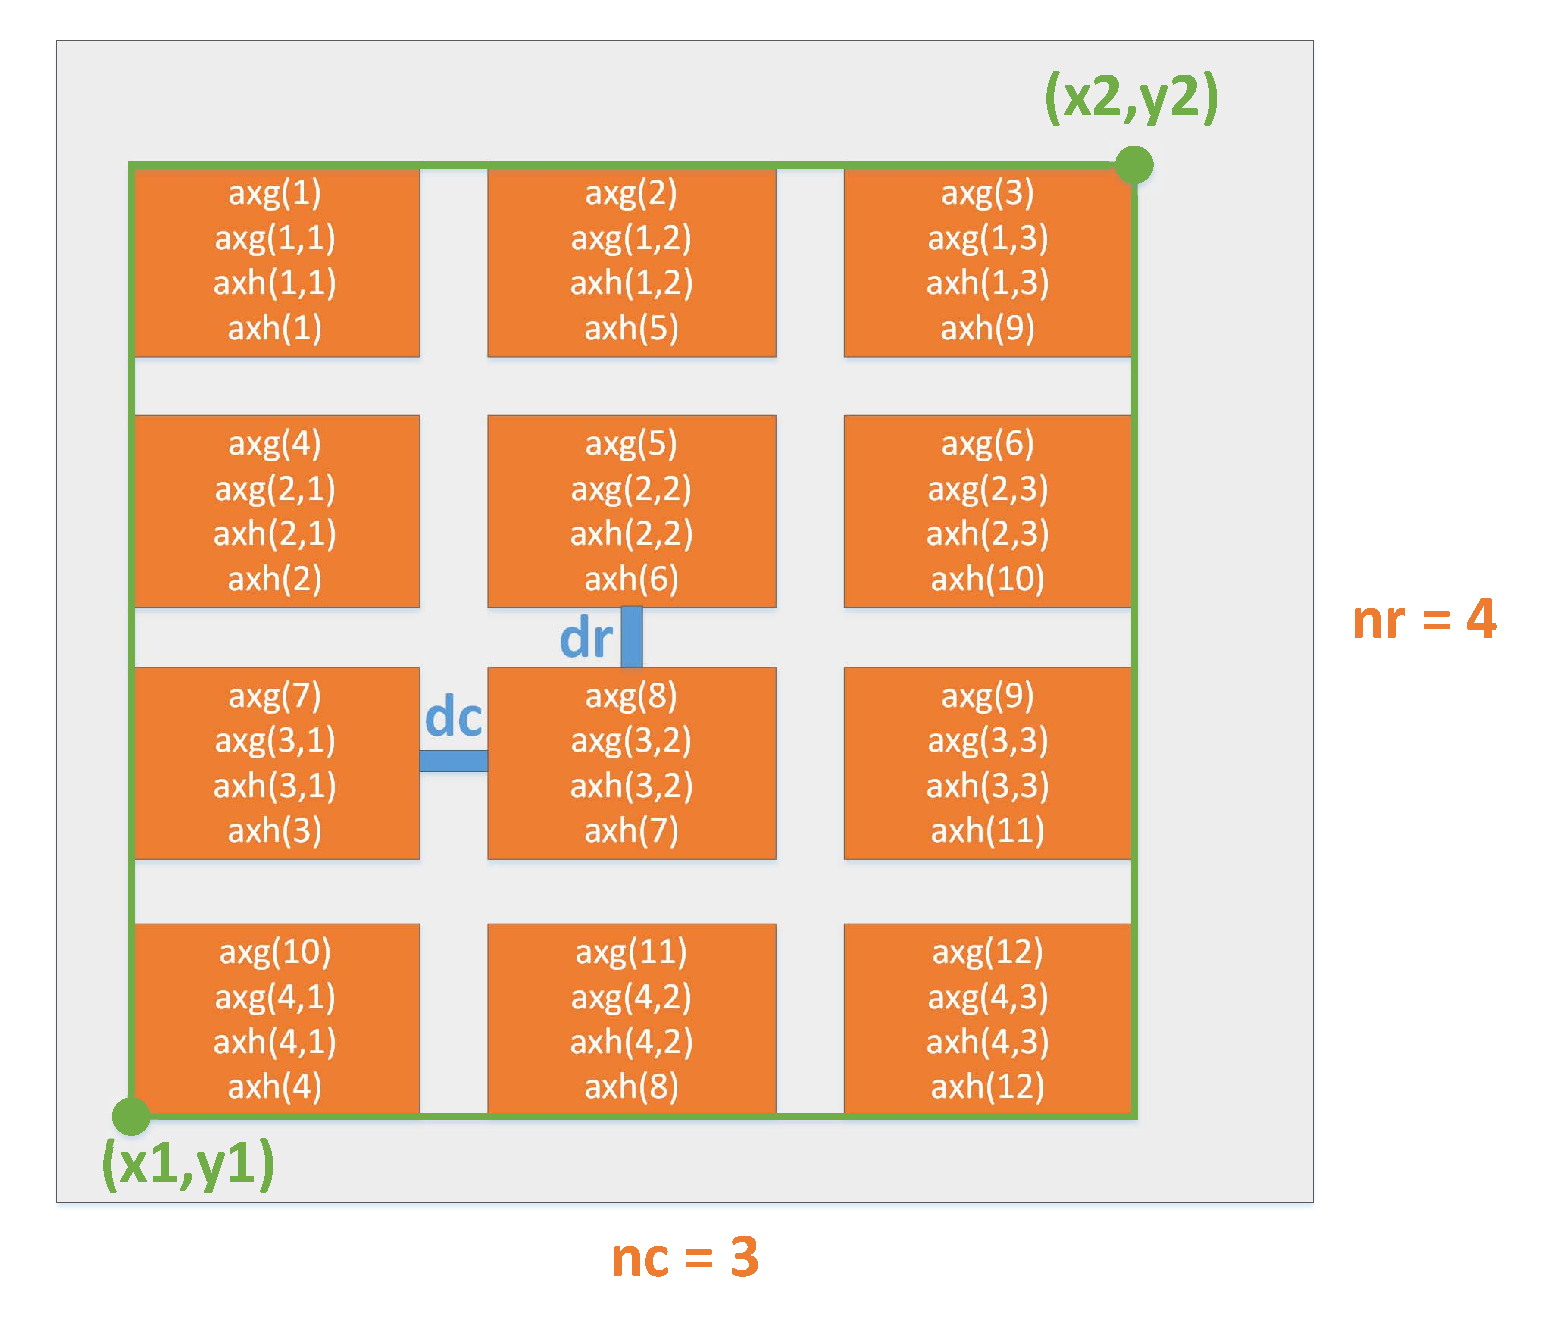
\includegraphics[height = \linewidth]{axgridDimensions}
	\end{figure}

	\clearpage
	\subsection*{Example Usage (\textit{exampleAxgrid.m})}
	\subsubsection*{Basic Preallocated Grid}

	\lstinputlisting[
	label      = {alg:lsr2},
	style      = Matlab-editor,
	basicstyle = \mlttfamily,
	firstline  = 1,
	lastline   = 12,
	firstnumber= 1
	]{../exampleaxgrid.m}
	
	\begin{figure}[H]
		\centering
		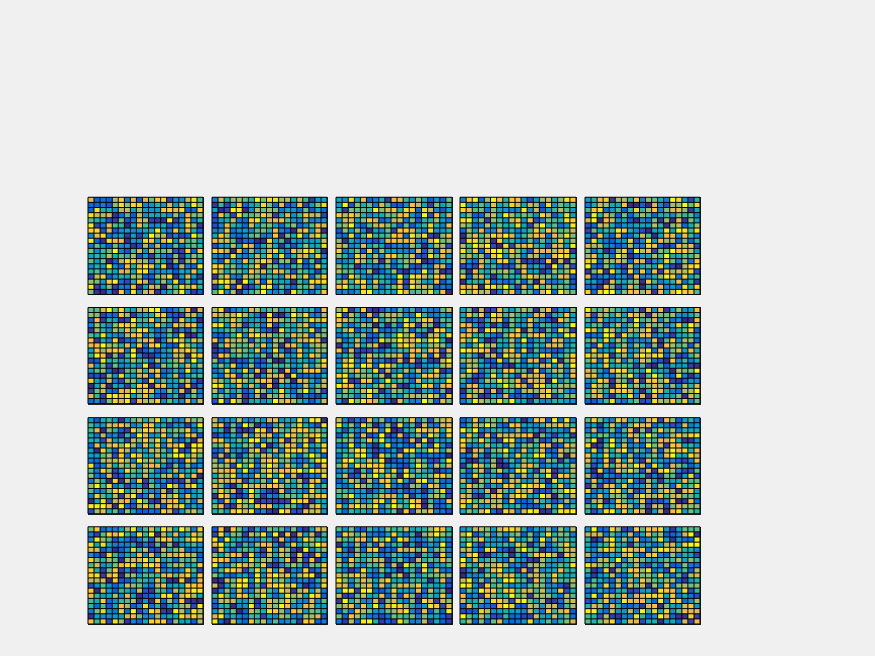
\includegraphics[height = 4in]{axgridex1}
	\end{figure}

	\clearpage
	\subsubsection*{Subplots use more than one grid cell}
	
	\lstinputlisting[
	label      = {alg:lsr2},
	style      = Matlab-editor,
	basicstyle = \mlttfamily,
	firstline  = 15,
	lastline   = 20,
	firstnumber= 15
	]{../exampleaxgrid.m}
	
	\begin{figure}[H]
		\centering
		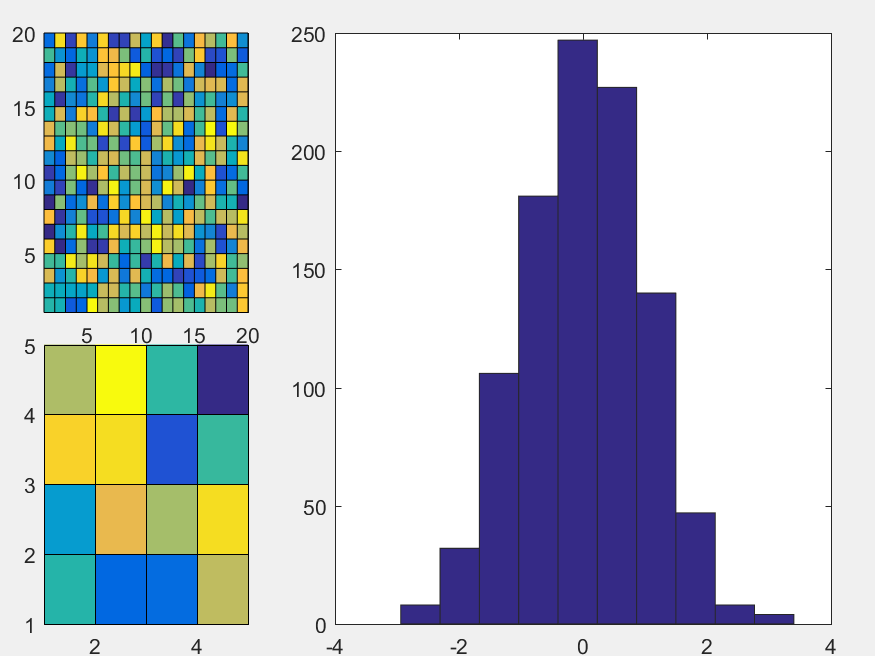
\includegraphics[height = 4in]{axgridex2}
	\end{figure}

	\clearpage
	\subsubsection*{Lots of subplots}
	
	\lstinputlisting[
	label      = {alg:lsr2},
	style      = Matlab-editor,
	basicstyle = \mlttfamily,
	firstline  = 24,
	lastline   = 39,
	firstnumber= 24
	]{../exampleaxgrid.m}
	
	\begin{figure}[H]
		\centering
		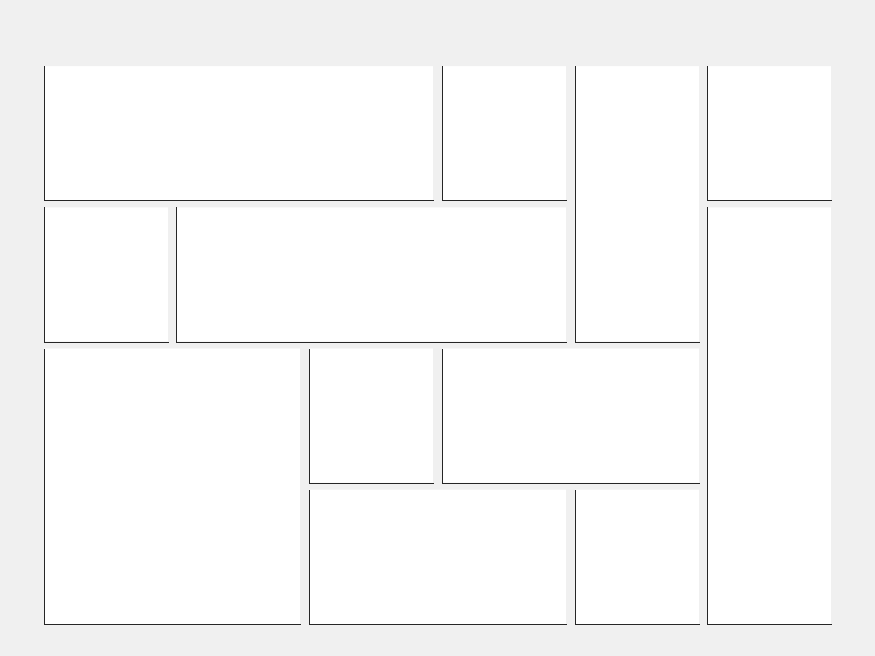
\includegraphics[height = 4in]{axgridex3}
	\end{figure}
	
	\clearpage
	\subsubsection*{Overlapping Subplots}
	You can get creative and overlap multiple subplots, making the top ones axes background invisible, and give each axes a different colormap.
	\lstinputlisting[
	label      = {alg:lsr2},
	style      = Matlab-editor,
	basicstyle = \mlttfamily,
	firstline  = 43,
	lastline   = 65,
	firstnumber= 43
	]{../exampleaxgrid.m}
	
	\begin{figure}[H]
		\centering
		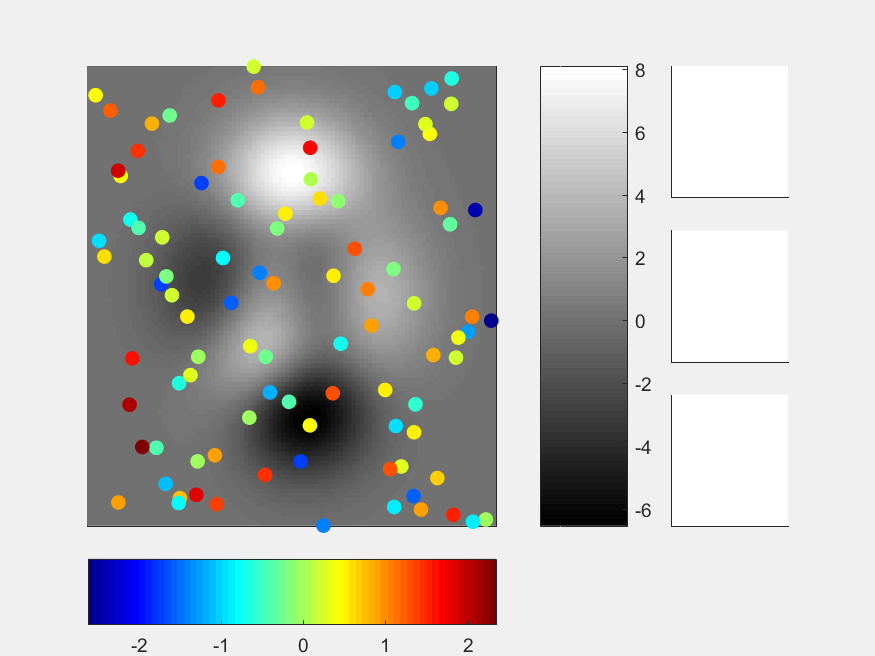
\includegraphics[height = 4in]{axgridex4}
	\end{figure}
\end{document}